\section{Evaluating Domain Platforms}
\label{sec:EvaOp}

To set the stage for our proposed domain DSE approach \newtext{(DSS and \ga)},
this sections introduces our assumptions / formalization about the
target platform in~\secref{sec:Platform}, \newtext{and different evaluation options of domain platform, Analytic Evaluation (AE)} in~\secref{sec:Ana} and Domain Score (DS) in~\secref{sec:ds}. ~\secref{sec:eva:sum} \newtext{discusses the accuracy and speed trade-off of these evaluation options.}

%\vspace{-4pt}
\subsection{Target Platform}
\label{sec:Platform}

To balance flexibility and efficiency, domain platform includes hardware accelerators (HWACC) and programmable processors (CPU, GPU, DSP), similar to current platforms. However, the number of HWACCs will increase dramatically, where individual HWACCs are less monolithic but smaller and configurable. HWACCs can be composed to accelerate larger kernels (or even applications), e.g. ACC-Rich MPSoCs \cite{cong2014accelerator} and FLP \cite{tabkhi2014function}. 

\begin{figure}[h]
	%\vspace{-4pt}
	\centering
	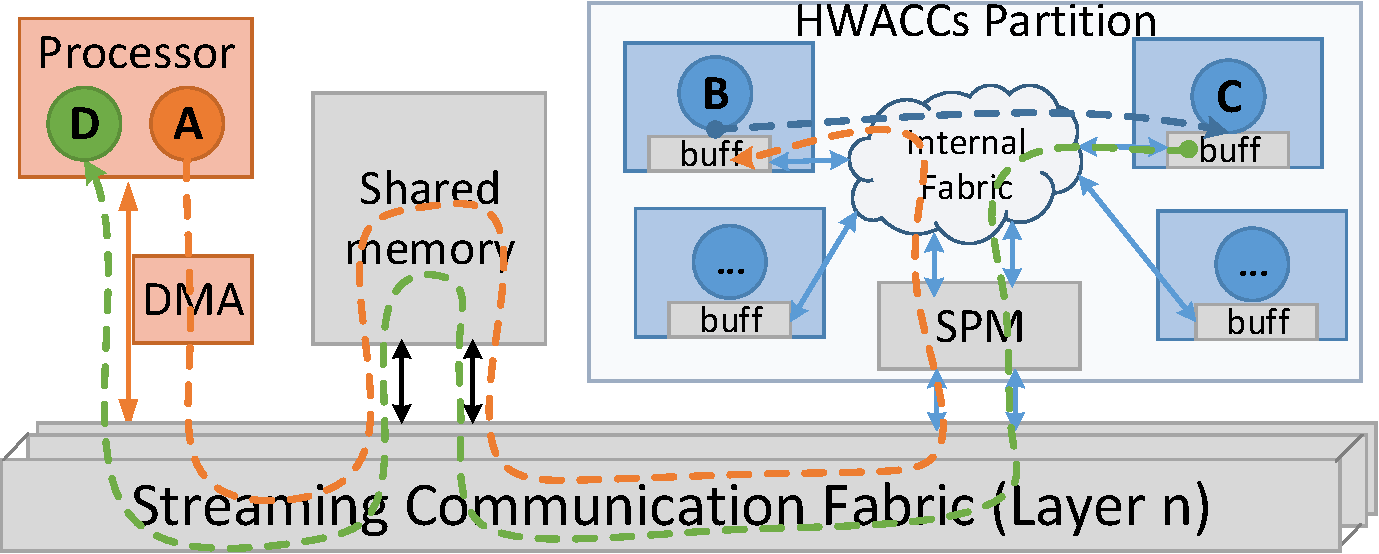
\includegraphics[width=.65\linewidth]{fig/pPlat.pdf}
	%\vspace{-6pt}
	\caption{Target Platform}
	\label{fig:plat}
	\vspace{-4pt}
\end{figure}

\figref{fig:plat} illustrates the target platform for the context of this work. A streaming application $A$,$B$,$C$,$D$ is mapped across SW and HW. Each HWACC has a dedicated SPM. All HWACCs are aggregated to a HW partition which a shared SPM across all HWACCs. HWACCs can communicate with each other; their communication traffic is hidden from system communication fabric (e.g. $B$, $C$). For simplicity, we assume direct n:n communication within the HW partition. Conversely, HWACCs and SW kernels communicate through the system streaming fabric (e.g. $A$ to $B$, and $C$ to $D$) which results in throughput penalties.


\newtext{Evaluating domain platforms is challenging due to the enormous design space needing to evaluate (a) the performance of each application given allocation and mapping, and (b) systematic aggregation across all applications to determine the platform benefit. For the purpose of this publication, we primarily focus on domain throughput improvement to assess the domain platform benefit. Domain throughput improvement is the average of all applications' throughput improvement each over their own pure SW implementation.} 

\newtext{Evaluating an individual application / platform follows a speed / accuracy trade-off. Transaction Level Models (TLM) can provide a reasonably high accuracy at cost of long simulation times limiting the number of evaluable design points in a given duration. More abstract and dramatically faster evaluation is desired to evaluate many more points at cost of accuracy.} 
~\secref{sec:Ana} and ~\secref{sec:ds} \newtext{propose two approaches and compares them against TLM simulation.}
\subsection{Analytic Evaluation}
\label{sec:Ana}

Performance analysis in context of DS-DSE is concerned about overall trends. Hence, the finer grained scheduling details of a TLM simulation are less important. As \ga targets streaming applications, the steady state performance is most important. 

The kernels in a streaming application operate as producers / consumers over the streaming data creating a pipeline. \figref{fig:Pipe} visualizes the pipeline execution for two HWACCs and one SW core. Each stage overlaps communication (in/out) with processing due to double buffering. Actors execute concurrently given their dependencies across different components. Actors mapped to the same component execute sequentially (e.g. in \emph{S8}).

Our analytical model computes the throughput of an application based on the inter-kernel pipelined execution~\cite{Teimouri_DAC_2015}.
At this abstraction, the throughput only depends on the pipe latency which is determined by the slowest processing component (or communication).

\begin{figure}[h]
	%\vspace{-10pt}
	\centering
	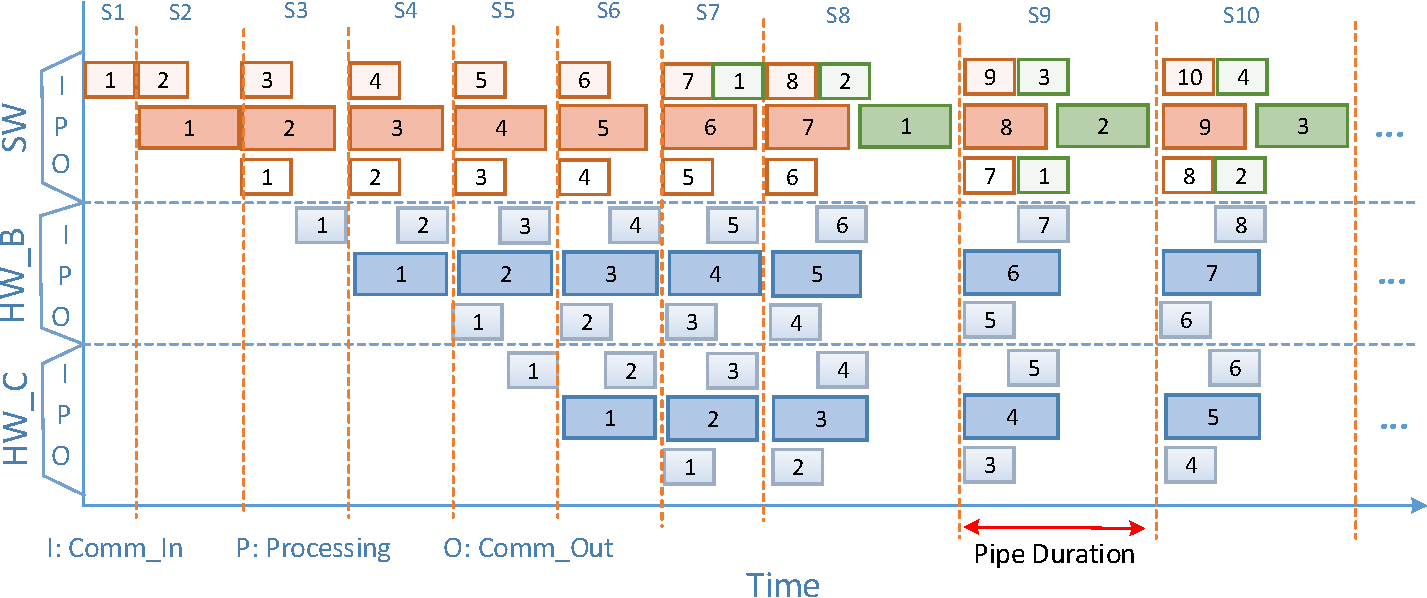
\includegraphics[width=\linewidth]{fig/pPipe.pdf}
	%\vspace{-10pt}
	\caption{Timing diagram of Architecture}
	\label{fig:Pipe}
	%\vspace{-6pt}
	
\end{figure}


Eq.~\eqref{eq:pipe} symbolically summarizes the analytical model. The estimated throughput is equal to output volume per iteration $D_{C}(out)$ over the pipe latency $L_{Pipe}$. \newtext{$L_{Pipe}$ is the maximum latency of SW ($L_{SW_i}$), HW ($L_{HW_j}$), and each layer of communication fabric ($L_{CE_k}$). }

\begin{equation}
\begin{split}
	&Throughput = D_{C}(out) / L_{Pipe} \\
	&L_{Pipe} = Max (\forall L_{SW}, \forall L_{HW}, \forall L_{CE}) \\
	&L_{SW_i} = \frac{\sum_{T \in SW_i} D_{P}(T)} {Freq_{SW}} + L_{sync} \\
	&L_{HW_j} = \frac{\sum_{T \in HW_j} D_{P}(T)} {Freq_{SW}*20} \\
	&L_{CE_k} = \frac{\sum_{C \in CE_k} D_{C}} {BW_{CE} * Freq_{CE}}
\label{eq:pipe}
\end{split}
\end{equation}

 \newtext{SW latency $L_{SW_i}$} is the accumulation of processing (i.e. total SW processing demand) and synchronization $L_{sync}$. Synchronization $L_{sync}$ is due to coordinating HW/SW communication including interrupt requests (from DMA, HW).
\newtext{HW latency $L_{HW_j}$} is due to processing an actor in HW. Each HWACC only executes one function type. 
The processing acceleration of an ACC depends on its frequency and the parallelism of the FT implemented on the ACC. For simplicity and clarity of explanation, this paper assumes a uniform HW acceleration of 20x. Non-uniform acceleration can be considered by defining an acceleration per function type.
\newtext{Communication latency $L_{CE_k}$} depends on the communication volume (between SW and HW) over bandwidth. Hence contention is only considered as an average. A multi-layer communication fabric is assumed. 
\subsection{Domain Score (DS)}
\label{sec:ds}

\newtext{For a rapid evaluation, an even higher abstraction level might be needed to gauge allocation / mapping benefits. For this, we develop the Domain Score (DS). Rather than estimating performance of an individual application on a platform, DS directly assesses costs and benefits of the platform to all applications in a domain.}
\newtext{DS relies on profiling all applications (only required once) to determine the total processing demand for each function type $D_P(t)$ and the communication demand between each function type pair $D_C(t_o,t_i)$. DS enables a relative comparison for incremental changes.} 
\newtext{DS quantifies the benefits of moving function types $t_{+}$ from SW to HW, and the penalties of moving $t_{-}$ from HW to SW with respect to processing and communication. In contrast to the analytic model, DS computes the score at once for the whole domain (i.e. incorporating all applications). No further aggregation and averaging are required.} 

%Given the amount of applications a domain and the myriad domain platform design options, a detailed simulations or detailed analytical approaches that include scheduling effects are prohibitively expensive to execute. Instead, our approach focuses on overall processing demand (i.e. how many operations) of the domain and processing supply by the architecture (symmetric for communication). The dynamic composition score quantifies the benefits moving a composition $C$ from processor to hardware mapping. DS estimates the benefits stemming from processing and communication mapping, scales them using dynamic weights (tuned to domain properties) and includes the additional cost of hardware implementation. 

%\vspace{-10pt}
\begingroup\makeatletter\def\f@size{9}\check@mathfonts
\begin{equation}
\begin{split}
\label{eq:scoreDS}
	Score &= B_{P} * w_{P} + B_{C} * w_{C}
	%cost &= \left\vert{C \cap SW}\right\vert
\end{split}
\end{equation}
\endgroup

In Eq.~\eqref{eq:scoreDS}, \newtext{$B_P$ and $B_C$ are the benefits of processing} and communication \newtext{when functions are changed in SW/HW mapping, respectively}. They are calculated considering aggregated benefits and appearances. $w_P$ and $w_C$ are the weights to scale both benefits. The weights are dynamically adjusted tracking performance bottlenecks, where processing or communication might be more important. Obtaining these weights will be discussed in Sec.~\ref{sub:weight}. %The $cost$ is defined the number of additional function types (i.e. HWACCs) to realize the composition in HW.


\subsubsection{Processing Benefit}
\label{sub:ben_proc}
Eq.~\ref{eq:comp} \newtext{estimates the processing benefit $B_P$ as execution time reduction / increase of the domain when mapping function types $t_{+}$ from SW to HW and $t_{-}$ from HW to SW, based on computation demand and supply.}

%\vspace{-10pt}
\begingroup\makeatletter\def\f@size{8.5}\check@mathfonts
\begin{equation}
\begin{split}
\label{eq:comp}
    B_{P} &= b_{P}(\{t_{+}\}) - b_{P}(\{t_{-}\}) \\
	b_{P}(X) &= \sum_{ t_{i} \in X } (\frac{D_{P}(t_{i})}{S_{SW}} - \frac{D_{P}(t_{i})}{S_{HW}}) * P(t_{i})
\end{split}
\end{equation}
\endgroup

In Eq.~\ref{eq:comp}, $S_{SW}$ and $S_{HW}$ are the estimated execution speed of SW and HW, respectively. \newtext{For each function type $t_{i}$ mapped from SW to HW, the overall difference of execution time between SW and and HW processing is calculated. This difference is then multiplied by the appearance probability $P$ of $t_{i}$ to prioritize frequently appearing compositions. The sum of the scaled processing benefits/disadvantage of these function types yields the processing benefit $B_P$ considering $t_{+}$ and $t_{-}$ switch.}
 
\subsubsection{Communication Benefit}
\label{sub:ben_comm}
The communication benefit is defined as the change in bus usage (transfer delay) due to switch mapping between sW and HW. It considers four aspects: \newtext{(1) $t_{+}$ saved communication with other HW-mapped functions, (2) $t_{+}$ additionally exposed HW/SW communication with other SW-mapped functions, (3) $t_{-}$ exposed SW/HW communication with other HW-mapped functions, and (4) $t_{-}$ saved communication with other SW-mapped functions. Communication between SW-mapped functions is assumed to be hidden in the memory hierarchy.} 

%\vspace{-10pt}
\begingroup\makeatletter\def\f@size{8.5}\check@mathfonts
\begin{equation}
\begin{split}
\label{eq:comm}
    B_{C} &=  b_{C}(\{t_{+}\}, HW \setminus \{t_{-}\}) - b_{C}(\{t_{+}\}, SW \setminus \{t_{+}\}) \\
        &- b_{C}(\{t_{-}\}, HW \setminus \{t_{-}\}) + b_{C}(\{t_{-}\}, SW \setminus \{t_{+}\}) \\
    b_{C}(X, Y) &= \sum_{ t_{i} \in X, t_{j} \in Y } D_{C}(t_{i},t_{j}) / S_{C} * P(t_{i},t_{j})
\end{split}
\end{equation}
\endgroup

Eq.~\eqref{eq:comm} captures the communication benefits, assuming $S_C$ is the communication speed of buses. It computes the saved versus exposed data transfer volume $D_C$ on bus divided by the communication speed $S_C$ to yield the change transfer delay. The change in delay scaling with appearance probability and its accumulation across all applications yields the communication benefit $B_C$, which is the change in transfer delay for the whole domain.


\subsubsection{Dynamic Weights}
\label{sub:weight}
Communication and processing demands vary by domains. In result, e.g. for a processing dominated domains (e.g. computer vision) targeting processing has priority resulting in the biggest improvements. While the benefits computed before already capture some of it, a global domain scope is needed to weigh the importance of communication versus processing of the whole domain. To capture this, we define the weights $w_C$ and $w_P$. 
However, each mapping to HW alters the effective communication vs. processing split and may change the properties and bottlenecks of the remaining compositions in a domain. For example, once processing intensive compositions are mapped to HW, the remaining compositions are communication-intensive. Therefore, the weights cannot be static but must be dynamically updated in each iteration to adjust for past mapping decisions.
%\vspace{-5pt}

\begingroup\makeatletter\def\f@size{8.5}\check@mathfonts
\begin{equation}
\begin{split}
\label{eq:weight}
	&w_{P} = \frac{\sum_{t_{i} \in SW} D_{P}(\{t_{i}\}) }{ \sum_{t_{i} \in SW} D_{P}(\{t_{i}\}) + \sum_{ \{t_{i}, t_{j}\} \nsubseteq HW} D_{C}(\{t_{i},t_{j}\}) }\\
	&w_{C} = 1 - w_P\\	
\end{split}
\end{equation}
\endgroup

Eq.~\eqref{eq:weight} illustrates the dynamic weight calculation. It uses the total remaining domain processing and communication demand (not mapped to HW) to determine the current performance bottleneck. A higher total demand of non-mapped (i.e. SW) processing raises the processing weight $w_P$. Conversely, if communication dominates the remaining domain, the communication demand $w_C$ will increase. 

%\secref{sub:dcs} and \secref{sec:GALS-DSS} will use the DS in the context of the Dynamic Score Selection (DSS) and GenetIc Domain Exploration (GIDE) algorithms. Since DSS greedily choosing the most promising function types $t_{+}$ for HW implementation, the DS only calculates the benefit of $t_{+}$ and the cost of consumed HW budget. However \ga comparing the switch of function types ($t_{+}$, $t_{-}$) implementation between SW and HW within certain budget, then DS considers the effect of both $t_{+}$ and $t_{-}$, and ignores the cost of budget consuming.

%\begingroup\makeatletter\def\f@size{8.5}\check@mathfonts
%\begin{equation}
%\begin{split}
%\label{eq:score}
%Score &= ( B_{P} * w_{P} + B_{C} * w_{C} )\\
%B_{P} &= D_{P}(t_{+}) - D_{P}(t_{-}) \\
%B_{C} &= \sum_{t_{I} \in HW}^{} D_{C}(t_{I}, t_{+}) - D_{C}(t_{I}, t_{-}) \\
%&+ \sum_{t_{I} \in SW}^{} D_{C}(t_{I}, t_{-}) - D_{C}(t_{I}, t_{+}) \\
%%B_{C} &= \sum_{t_{I} \in HW}^{} ( D_{C}(t_{I}, t_{+}) - D_{C}(t_{I}, t_{-}) ) + \sum_{t_{I} \in SW}^{} ( D_{C}(t_{I}, t_{-}) - D_{C}(t_{I}, t_{+}) )\\
%w_{P} &= \frac{\sum_{t_{I} \in SW} D_{P}(\{t_{I}\}) }{ \sum_{t_{I} \in SW} D_{P}(\{t_{I}\}) + \sum_{ \{t_{I}, t_{J}\} \nsubseteq HW} D_{C}(\{t_{I},t_{J}\}) }\\
%w_{C} &= 1 - w_P
%\end{split}
%\end{equation}
%\endgroup


\subsection{Trade-off: Evaluation Speed / Accuracy }
\label{sec:eva:sum}

To compare the the evaluation approaches in terms of accuracy and speed, we analyze them for a set of 40 real vision applications on 100 different platforms (with the same HW budget=5) against execution on a cycle-approximate TLM. % please name the few
\tabref{tab:fidelity} illustrates the trade-off looking at fidelity instead of accuracy as the evaluation approaches are compare design alternatives. TLM is defined as 100\% fidelity for this comparison.

\begin{table}[h]
	\caption{Fidelity and Speed: DS, \newtext{AE}, TLM}
	\label{tab:fidelity}
	\centering
	%\vspace{-10pt}
	\begin{tabular}{r||c|c|c}
		\toprule
		  & \textbf{DS}& \textbf{AE}& \textbf{TLM}\\
		\hline
		\midrule
		\textbf{Fidelity} & 89.07\%& 95.68\%& 100\%\\
		\hline
		\textbf{Eval. App [s]} & $7.2*10^{-5}$ & $6.0*10^{-4}$ & $1.8*10^2$ \\
		\hline
		\textbf{Eval. Domain [s]} & $7.2*10^{-5}$ & $6.0*10^{-2}$ & $1.8*10^4$ \\
		\bottomrule
	\end{tabular}
\end{table} 

Fidelity drops with abstraction: AE with 95.68\% and DS with 89.07\%. At the same time, abstraction yields dramatic speedups of 6 orders of magnitude from TLM to AE and another order of magnitude to DS. When evaluating a whole domain, DS is even 3 orders of magnitude faster than AE (assuming 100 apps in the domain) due to inherently incorporating all applications. In result, DS is preferred for rapid analysis, whereas the AE if more accuracy is needed. TLM simulation is too slow for DS-DSE.